\begin{posterblock}{white}{smunavy}{smublue}{smulight}{Introduction}
\begingroup
\fontsize{24.0}{29.0}\selectfont
\setlength{\parskip}{1.0ex}
Large-scale liquid hydrogen (LH$_2$) cargo containment requires thin metallic barriers that remain gas-tight while absorbing thermal contraction and restrained in-plane displacement. Our previous numerical design work identified an orthogonally corrugated 316L stainless-steel membrane as a candidate barrier: the corrugations redirect global contraction into local bending, lowering strain demand in the planar sheet under LH$_2$ thermal-contraction and pressure-difference load cases.

This poster turns that design claim into an experimental validation route. Formed specimens are evaluated by digital image correlation (DIC) tensile testing to observe strain redistribution and by acoustic emission (AE) monitoring during cyclic loading to screen damage evolution; a 0.2~m$^3$ membrane demonstrator is then cycled in liquid nitrogen (LN$_2$) with pressure-retention and leak-check assessment. Because hydrogen-rated mechanical testing requires dedicated safety infrastructure, room-temperature tests isolate the geometry-driven deformation mechanism while LN$_2$ cycling provides a non-flammable cryogenic integrity screen before future LH$_2$ qualification.

\vspace{0.8ex}
\begin{columns}[t,totalwidth=\linewidth]
\begin{column}[t]{0.36\linewidth}
\vspace{0pt}
\begin{minipage}[t][\introvisualheight][s]{\linewidth}
\centering
\introfiguretitle{(A) Membrane-type storage tank}
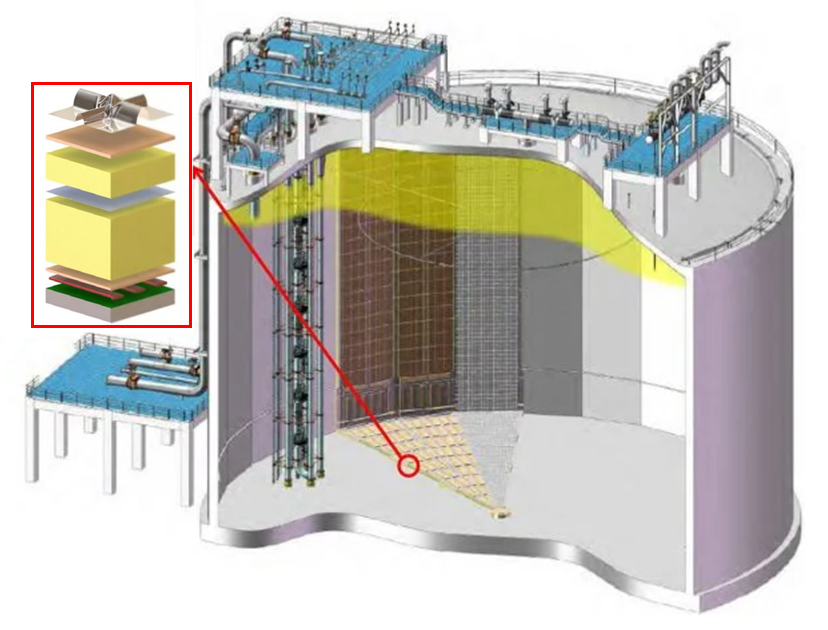
\includegraphics[width=\linewidth,height=9.5cm,keepaspectratio]{assets/membrane_type_storage_tank.png}

\vfill
\introfiguretitle{(B) Corrugated membrane geometry}
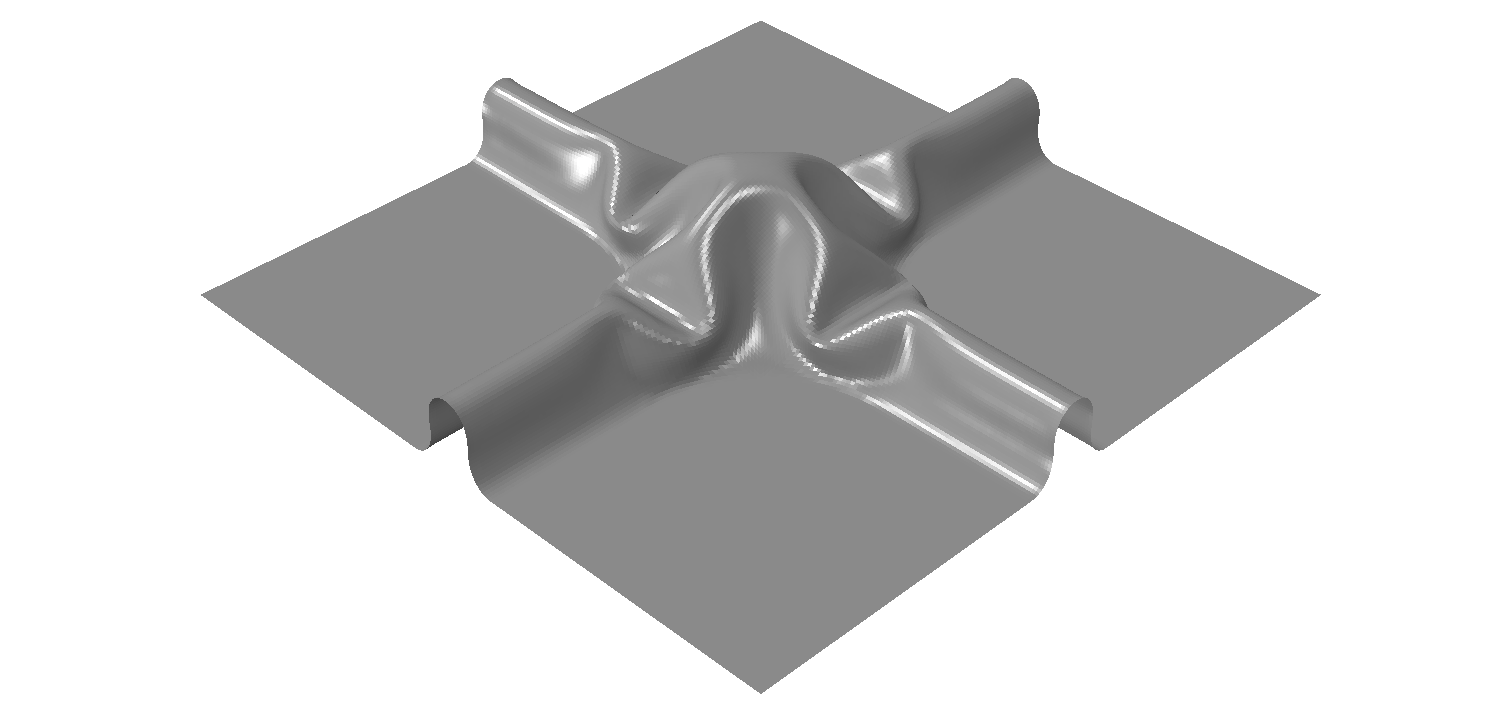
\includegraphics[width=\linewidth,height=6.0cm,keepaspectratio]{assets/membrane.png}
\end{minipage}
\end{column}
\hfill
\begin{column}[t]{0.62\linewidth}
\vspace{0pt}
\begin{minipage}[t][\introvisualheight][s]{\linewidth}
\centering
\introfiguretitle{(C) Experimental validation route}
\resizebox{\linewidth}{!}{% ---------- Panel C: Validation route ----------
\begin{tikzpicture}[
    font=\rmfamily,
    method/.style={
        draw=black!70,
        rounded corners=3pt,
        line width=0.55pt,
        fill=white,
        text width=8.20cm,
        minimum height=1.35cm,
        align=center,
        inner xsep=4pt,
        inner ysep=5pt,
        font=\rmfamily\scriptsize
    },
    purpose/.style={
        draw=black!70,
        rounded corners=3pt,
        line width=0.55pt,
        fill=white,
        text width=6.20cm,
        minimum height=1.35cm,
        align=center,
        inner xsep=4pt,
        inner ysep=5pt,
        font=\rmfamily\scriptsize
    },
    header/.style={
        font=\rmfamily\bfseries\scriptsize,
        align=center
    },
    rowarrow/.style={
        -{Latex[length=1.8mm,width=1.2mm]},
        line width=0.45pt,
        black!55
    },
    downarrow/.style={
        -{Latex[length=2.0mm,width=1.35mm]},
        line width=0.50pt,
        black!70
    }
]

\node[header] at (0,0) {Method};
\node[header] at (8.35,0) {Purpose};

\node[method] (m0) at (0,-1.45)
{\textbf{Fabrication}\\
Controlled forming of 316L sheet\\
Corrugated specimen preparation};

\node[method] (m1) at (0,-3.45)
{\textbf{DIC-instrumented tensile test}\\
Four-axis cyclic stretching\\
Full-field strain measurement};

\node[method] (m2) at (0,-5.45)
{\textbf{AE-instrumented tensile test}\\
Four-axis cyclic stretching\\
Acoustic emission monitoring};

\node[method] (m3) at (0,-7.45)
{\textbf{LN$_2$ cycling test}\\
Assembled membrane structure\\
Filling--draining cycles};

\node[purpose] (p0) at (8.35,-1.45)
{Obtain target\\
corrugated specimens\\
and membrane modules};

\node[purpose] (p1) at (8.35,-3.45)
{Quantify full-field\\
strain redistribution};

\node[purpose] (p2) at (8.35,-5.45)
{Track damage evolution\\
during cyclic loading};

\node[purpose] (p3) at (8.35,-7.45)
{Verify assembly integrity\\
after cryogenic cycling};

\foreach \m/\p in {m0/p0,m1/p1,m2/p2,m3/p3}{%
    \draw[rowarrow] (\m.east) -- (\p.west);
}

\draw[downarrow] (m0.south) -- (m1.north);
\draw[downarrow] (m1.south) -- (m2.north);
\draw[downarrow] (m2.south) -- (m3.north);

\end{tikzpicture}
}
\vfill
\end{minipage}
\end{column}
\end{columns}
\endgroup
\end{posterblock}
